\documentclass[fleqn]{ic-relatorio}
\usepackage{relatorio}
\usepackage{booktabs}
\usepackage{multirow}
\usepackage{longtable}
\usepackage{float}
\usepackage{url}
\usepackage{listings}
\usepackage{color}
\usepackage{amsthm}
\addbibresource{refs.bib}

\title{ULP Transitions, Rounding, and Absorption in $(x^{10}+c)-x^{10}$: A Study of IEEE 754 Binary32 and Binary64}
\autor{Enzo Rocha Leite Diniz Ribas}
\date{\today}
\orientador{Lucas Martins Rocha}
\coorientador{Luis Alberto D'Afonseca}


\newcommand{\fl}{\operatorname{fl}}
\newcommand{\ulp}{\operatorname{ulp}}
\newcommand{\rnd}{\operatorname{RN}}
\newcommand{\nuval}{\nu(c)}
\newcommand{\F}{\mathbb{F}}
\newcommand{\code}[1]{\texttt{\detokenize{#1}}}
\newtheorem{proposition}{Proposition}[chapter]
\newtheorem{corollary}[proposition]{Corollary}
\newtheorem{remark}[proposition]{Remark}
\newtheorem{lemma}[proposition]{Lemma}
\setlength{\emergencystretch}{2em}



\begin{document}
\begin{Abstract}
In exact arithmetic, the expression $(x^{10}+c)-x^{10}$ is identically equal to $c$. In finite-precision binary arithmetic, however, its computed value displays a sequence of plateaus, parity-dependent rounding ties, and eventually complete absorption of the increment. This report investigates that behavior in IEEE 754 \code{binary32} and \code{binary64}, using the supplied research manuscript, extended book draft, experimental report, notebook, and interactive graphics. Writing $y=\fl(x^{10})$, $u=\ulp(y)$, and $c=m2^{\nu}$ for odd $m$, the nearest-grid model predicts an initial inexact binade at $E_1=p+\nu$ and the last potentially nonzero binade at $E_2=p+\lfloor\log_2 c\rfloor$, where $p$ is significand precision. Consequently, the predicted inexact interval in $x$ is approximately $[2^{(p+\nu)/10},\,2^{(p+1+\lfloor\log_2 c\rfloor)/10})$ and spans $L=\lfloor\log_2 c\rfloor-\nu+1$ binades. The model is established under explicit assumptions about rounding, reuse of the computed power, and binade boundaries. Results reported in the supplied study cover 1,611 values of $c$ in each precision and distinguish powers of two, odd integers, dyadic fractions, and non-dyadic decimal or reciprocal inputs. Reconstructed visualizations and an independently checked 780-case power-of-two grid illustrate when increments are preserved, rounded, or absorbed. Special attention is given to boundary effects, input representation, the relation to Fast2Sum, and limitations of the model.

\Keywords IEEE 754; floating-point arithmetic; unit in the last place; rounding to nearest; cancellation; absorption; binary32; binary64; numerical reproducibility.
\end{Abstract}

\tableofcontents
\listoffigures
\listoftables

\chapter{Introduction}\label{ch:intro}

\section{Motivation}
The mathematical identity
\begin{equation}\label{eq:real}
 (x^{10}+c)-x^{10}=c
\end{equation}
holds for every real $x$ and $c$. Its evaluation in floating-point arithmetic, however, does not necessarily return $c$. The first addition may round away part or all of the increment, even when the subsequent subtraction is itself exact. As the magnitude of $x^{10}$ grows, the gap between representable numbers grows in discrete steps. This makes Equation~\eqref{eq:real} a compact way to observe rounding, absorption, and cancellation-related loss of information \cite{goldberg1991floating,higham2002accuracy}.

The central quantity is the \emph{unit in the last place} (ULP). Unlike a fixed absolute error tolerance, the ULP changes with the exponent of the stored floating-point number. An increment that is easily represented near one magnitude may lie exactly halfway between two representable results at a larger magnitude, then become too small to change the larger operand at all. The behavior is therefore not accurately described by a single threshold in $x$ for every possible increment $c$.

\section{Research question and aims}
This report addresses the question: \emph{How do the magnitude and binary bit structure of a positive floating-point increment $c$ determine the first rounding error, the intermediate output values, and complete absorption in $(x^{10}+c)-x^{10}$?}

The specific aims are to describe a common model for four families of increments, connect its thresholds to IEEE 754 precision, present empirical results and figures from the supplied sources, and separate established mathematical statements from experimental observations and still-open questions. The expression is treated as a study of floating-point evaluation rather than as a proposal for a new numerical algorithm.

\section{Contributions and provenance}\label{sec:provenance}
The manuscript by Rocha dated 4 November 2026 provides a piecewise nearest-grid model, formulas for the two transition thresholds, and results for 1,611 increments in each of two precisions \cite{rocha2026manuscript}. The accompanying extended draft develops proofs, reviews related error-free transformations, and identifies qualifications to the binade-wise description. A separate seven-page experimental report and the \code{ulp.ipynb} notebook supply plots and a focused enumeration of negative powers of two. Four supplied Plotly HTML charts visualize the power-of-two, odd-integer, and fractional cases.

This document reorganizes these materials into an English-language report while preserving the distinction between the published mathematical framework of floating-point rounding and the particular threshold notation used in the supplied project. The figures are regenerated in English from equivalent NumPy experiments; the plotting script is included. The full source files supplied by the author remain the primary evidence for the larger-scale experiments, and large-scale validation counts are reported as source claims rather than as experiments rerun for this report.

\section{Scope and assumptions}
The analysis principally considers finite, positive, normal operands in IEEE 754 \code{binary32} (precision $p=24$) and \code{binary64} ($p=53$) \cite{ieee7542019}. Operations round to nearest, with ties resolved toward an even least-significant significand bit. The power $x^{10}$ is evaluated once and its stored result $y$ is reused in the addition and subtraction. No fused evaluation, extended-precision intermediate, overflow, or underflow is assumed in the central argument. Most exact statements additionally require $y\ge c$ and require that the exact sum $y+c$ remain within the binade of $y$. These qualifications matter in interpreting early fractional results and samples close to powers of two.

\section{Organization}
Chapter~\ref{ch:theory} introduces floating-point representation and derives the nearest-grid rule and thresholds. Chapter~\ref{ch:method} records the experimental setup and source datasets. Chapter~\ref{ch:results} reports observations, numeric tables, and visualizations. Chapter~\ref{ch:discussion} discusses exceptions, error-free transformations, and practical consequences; Chapter~\ref{ch:conclusion} concludes. Appendix~\ref{app:rep} supplies reproducibility instructions and notes about the source archives.

\chapter{Theoretical Framework}\label{ch:theory}

\section{Binary floating-point spacing}
A normal binary floating-point number of precision $p$ can be written
\begin{equation}\label{eq:float}
 y=M\,2^{E-p+1},\qquad 2^{p-1}\le M<2^p,\quad M\in\mathbb{Z},
\end{equation}
where $E=\lfloor\log_2 y\rfloor$ is the binade exponent. If $y\in[2^E,2^{E+1})$, the upward spacing throughout the interior of that binade is
\begin{equation}\label{eq:ulp}
 u=\ulp(y)=2^{E-p+1}.
\end{equation}
The spacing is constant within each binade and doubles at the next power of two. For binary64, the transition from $u=1$ to $u=2$ occurs at $y=2^{53}$; when $y\approx x^{10}$, this corresponds to $x\approx2^{53/10}\approx39.3966$. In binary32, the analogous transition is at $x\approx2^{24/10}\approx5.2780$.

\begin{figure}[htbp]
\centering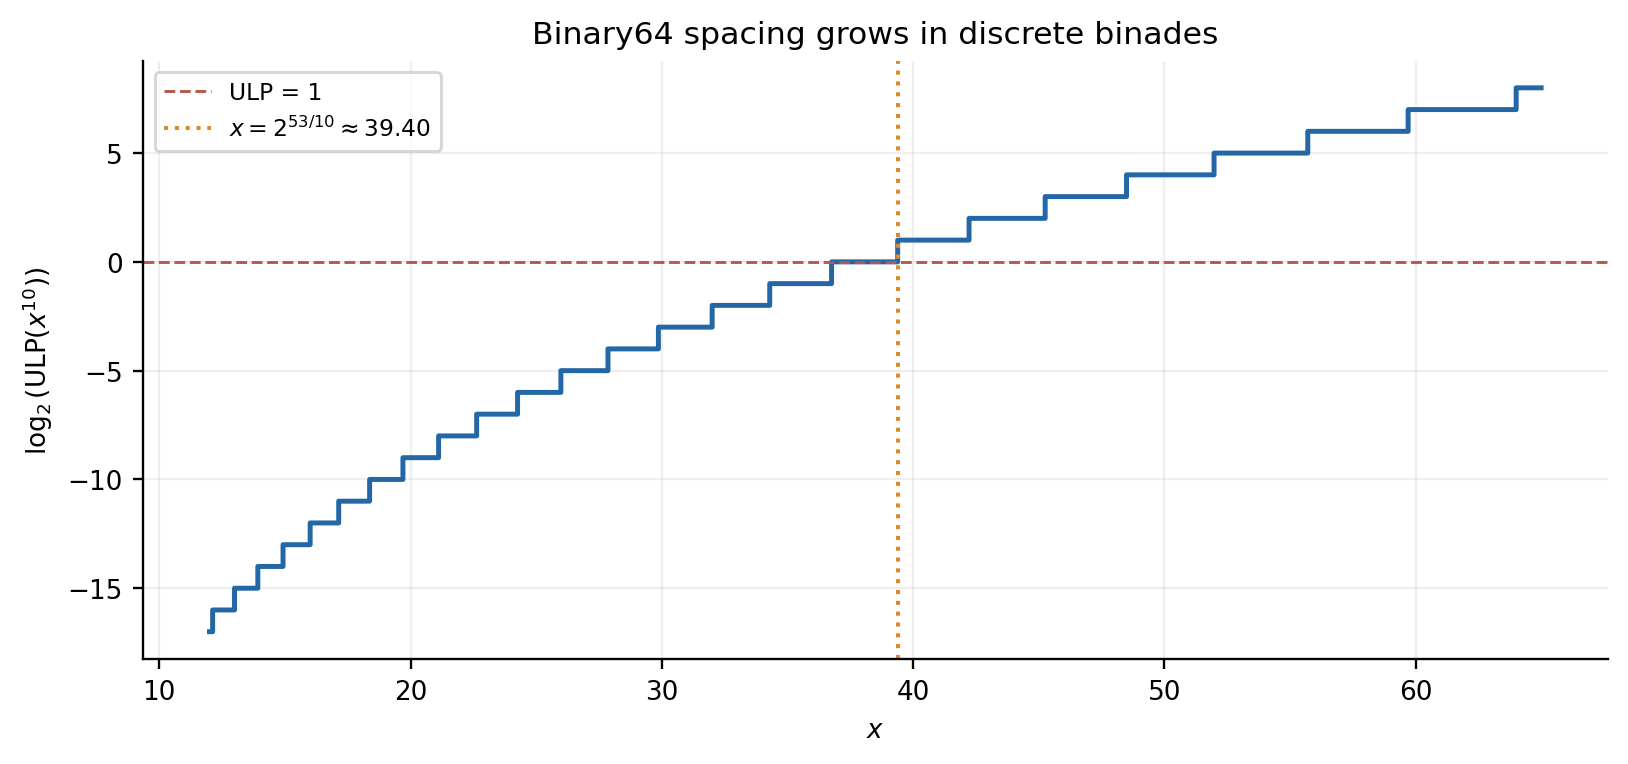
\includegraphics[width=.91\textwidth]{figs/01_ulp_staircase.png}
\caption{Reconstructed binary64 ULP staircase for $x^{10}$. The dashed line marks $u=1$, and the dotted line marks the $u=2$ transition.}\label{fig:ulp}
\end{figure}

\section{The computed function and exact final subtraction}
Let
\begin{equation}\label{eq:fn}
 y=\fl(x^{10}),\qquad s=\fl(y+c),\qquad f(x;c)=\fl(s-y).
\end{equation}
A central fact is that the subtraction in Equation~\eqref{eq:fn} need not introduce an additional error. Under $y\ge c>0$ and normal finite arithmetic, $s$ is sufficiently close to $y$ for the subtraction to be exact by Sterbenz's lemma (which states that $a-b$ is exactly representable when two floating-point operands satisfy $b/2\le a\le2b$ under the usual exponent-range hypotheses) \cite{sterbenz1974floating,higham2002accuracy}. Thus $f=s-y$ and the local error arises from the rounded addition.

Write the positive stored increment in lowest binary terms as
\begin{equation}\label{eq:nu}
 c=m2^{\nu},\qquad m\text{ a positive odd integer},\quad
 \lambda=\lfloor\log_2 c\rfloor.
\end{equation}
Here $\nu=\nu(c)$ is the exponent of the least significant nonzero bit in the exact stored value of $c$. This is meaningful even when the user typed a non-dyadic decimal: the stored binary32 or binary64 number is always dyadic.

\section{Nearest-grid rule and ties}
\begin{proposition}[Binade-wise rounding model]\label{prop:grid}
Assume round-to-nearest, ties-to-even; $y\ge c>0$; reuse of the same stored $y$; and $y+c<2^{E+1}$, so the exact sum remains in the same binade. Set $u=2^{E-p+1}$, $M=y/u\in\mathbb{Z}$, and $q=c/u$. Then
\begin{equation}\label{eq:grid}
 f(x;c)=u\,k,\quad k=\begin{cases}
 q, & q\in\mathbb{Z},\\
 \lfloor q+\tfrac12\rfloor,&q\notin\mathbb{Z}+\tfrac12,\\
 \text{the integer in }\{\lfloor q\rfloor,\lceil q\rceil\}
 \text{ for which }M+k\text{ is even}, &q\in\mathbb{Z}+\tfrac12.
 \end{cases}
\end{equation}
\end{proposition}
\begin{proof}
The stored $y=Mu$ is a point on the binade's representable grid. Rounding $y+c=u(M+q)$ to nearest selects $s=u(M+k)$, with ties resolved by even $M+k$. Sterbenz's lemma makes the final subtraction exact, yielding $f=s-y=uk$.
\end{proof}

In particular, all ties depend on the parity of the stored significand $M$, not only on the magnitude of $c$. For example, at $x=40$ in binary64, $y=40^{10}=10{,}485{,}760{,}000{,}000{,}000$ is exactly representable, $u=2$, and $M$ is even. Thus $c=1$ gives $f=0$, $c=3$ gives $f=4$, and $c=5$ gives $f=4$. A neighboring stored $y$ with odd $M$ can select the other side of a tie.

\section{Thresholds and the width of the inexact region}
\begin{proposition}[Transition binades]\label{prop:thresholds}
Under the hypotheses of Proposition~\ref{prop:grid}, let
\begin{equation}\label{eq:bounds}
 E_1=p+\nu,\qquad E_2=p+\lambda,\qquad
 L=E_2-E_1+1=\lambda-\nu+1.
\end{equation}
Below $E_1$, the grid resolves $c$ exactly. At $E_1$, the increment lies exactly halfway between two grid points and the result alternates between $c-u/2$ and $c+u/2$ according to parity. In subsequent binades through $E_2$, the rounded increment is a binade-dependent multiple of $u$; above $E_2$ it is zero. Consequently, in terms of $x$ the predicted transition interval is approximately
\begin{equation}\label{eq:xthreshold}
 x_1=2^{(p+\nu)/10},\qquad
 x_2=2^{(p+1+\lambda)/10},\qquad
 \frac{x_2}{x_1}=2^{L/10}.
\end{equation}
These are thresholds in the exponent of the \emph{computed} $y$; their numerical $x$ locations may shift slightly because $y=\fl(x^{10})$ and because of finite input sampling.
\end{proposition}
\begin{proof}
If $u\le2^{\nu}$, the power-of-two grid spacing divides $c=m2^{\nu}$, so $c/u$ is an integer and Equation~\eqref{eq:grid} returns $c$. The first larger spacing is $u=2^{\nu+1}$, where $q=m/2$ is a half-integer. For still larger powers of two, $q$ is neither integral nor halfway between consecutive integers. The rounded result becomes identically zero once $u>2c$, i.e., for exponents $E>p+\lambda$. The number of potentially inexact binades is therefore $L=(p+\lambda)-(p+\nu)+1$. The conversion from exponents of $y\approx x^{10}$ produces Equation~\eqref{eq:xthreshold}. If $c$ is itself a power of two, the final tie binade can yield either zero or $2c$; the fully absorbed regime starts in the following binade.
\end{proof}

The integer $L$ is the binary bit length of the odd significand $m$. For $c=2^j$, $L=1$. For positive odd integers, $\nu=0$ and $L=\lfloor\log_2 c\rfloor+1$. For typical stored approximations to non-dyadic fractions, $L$ is close to the full precision $p$.

\section{Error measured in ULPs}
Whenever Proposition~\ref{prop:grid} applies, the normalized error is
\begin{equation}\label{eq:eps}
 \varepsilon=\frac{f-c}{u}=k-q,\qquad |\varepsilon|\le\frac12.
\end{equation}
Thus the absolute error is bounded by half a ULP \emph{of $y$} in the stated regime. The bound is not a guarantee of small \emph{relative} error: $(f-c)/c$ can reach $-1$ under complete absorption, and can be appreciable even before that point.
\begin{figure}[htbp]
\centering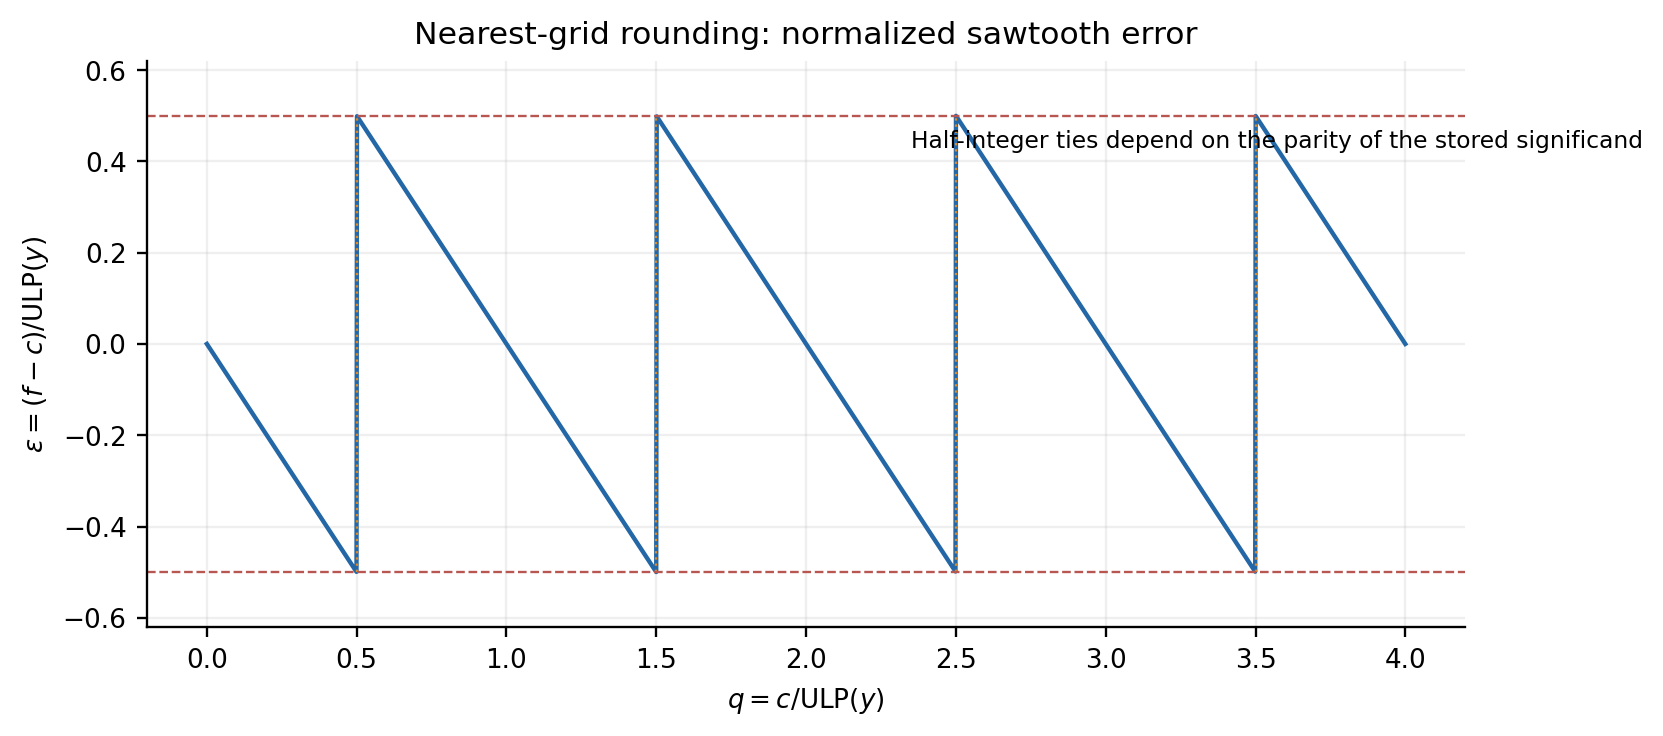
\includegraphics[width=.83\textwidth]{figs/08_ulp_sawtooth.png}
\caption{Theoretical normalized rounding error as a function of the increment measured in ULPs. Values at half-integer ties require the parity rule.}\label{fig:sawtooth}
\end{figure}

\section{Qualifications at binade borders and for \texorpdfstring{$y<c$}{y less than c}}\label{sec:exceptions}
At the upper edge of a binade, $y+c$ may cross into the next binade, where the spacing is $2u$. The fixed-$u$ nearest-grid formula then requires modification. The supplied extended manuscript gives a bound of $|f-c|\le u$ for this crossing case when $y\ge c$, instead of the interior bound $u/2$ \cite{rocha2026bookdraft}.

For $y<c$, the final subtraction need not satisfy Sterbenz's hypotheses, and the same manuscript provides a broader bound $|f-c|\le2\ulp(c)$ with a proof sketch. It reports the stronger empirical observation $|f-c|\le\ulp(c)$ in tested samples, but does not claim to have proved that stronger statement. Neither phenomenon should be hidden by interpreting Equation~\eqref{eq:xthreshold} as a universal exact classification for every $x$.

\chapter{Experimental Design and Reproduction}\label{ch:method}

\section{Data sources and original computational design}
The principal inputs are the supplied eight-page research manuscript, its 42-page book-length draft, the seven-page preliminary report, the original \code{ulp.ipynb} notebook, four Plotly HTML exports, and the associated source-code archive. The preliminary report investigates $c=2^{-k}$, $k=1,\ldots,20$, and $c$ from two further families: odd integers and reciprocals of odd denominators. The manuscript and book draft extend these investigations to a systematic precision-dependent model.

The supplied validation code specifies three types of $c$, for each of binary64 and binary32: 1,001 odd integers from $1$ to $2,001$; 300 generated dyadic fractions; and 310 non-dyadic inputs consisting of ten named constants or fractions and 300 sampled real inputs. These categories total \textbf{1,611 increments per precision}. The stated random generator is \code{numpy.random.default_rng(42)}. The code samples 1,500--4,000 values of $x$ per relevant binade, computes $y=x^{10}$, stores $y$ once, and evaluates $(y+c)-y$. Results are grouped using the actual exponent of the computed $y$, with samples for which $y+c$ crosses a binade border handled separately.

\section{Floating-point conventions}
Arithmetic results are compared at the precision used for each experiment. The binary64 experiments use NumPy's \code{float64}, while binary32 experiments cast both $x$ and $c$ to \code{float32} before arithmetic to avoid unintentional promotion. Given a finite value $y$, the upward ULP in the numerical experiments is obtained from
\begin{equation}\label{eq:nextafter}
 \ulp(y)=\code{nextafter}(y,+\infty)-y.
\end{equation}
For every sample the recorded quantities are the increment $c$, the actual $y$, the result $f$, its relative error $(f-c)/c$, and (where applicable) its ULP-scaled error $(f-c)/\ulp(y)$.

\section{Focused replication and figure generation}
A smaller deterministic check was independently executed during report preparation: $x$ takes the 39 integers from $2$ through $40$, while $k$ takes the 20 integers from $1$ through $20$, with $c=2^{-k}$ and binary64 arithmetic. The 780 results are classified as preserved, absorbed, tied downward, or tied upward. The resulting counts match the supplied preliminary report and are given in Table~\ref{tab:powercount}.

All included visualizations are generated by \code{scripts/generate\_figures.py}, which performs the arithmetic again with NumPy and saves static PNG plots with English axes and captions. The power-of-two map, continuous curves, odd-integer curves, and odd-reciprocal curves are counterparts of the four supplied interactive HTML exports. Additional plots recreate the ULP staircase, precision comparison, odd-integer error map, and the model's normalized rounding pattern described in the research manuscript. The original interactive HTML is not directly embedded in the PDF, since its interface labels and tooltips are in Portuguese and interactive JavaScript is not portable in a conventional LaTeX PDF.

\section{Reproducibility and evidential status}
The figures and the 780-case enumeration were regenerated locally. The 1,611-per-precision validation outcome, large-scale binade-border frequencies, and the original source tables are reported from the supplied study and were \emph{not} rerun at their full sample sizes in this document. This distinction is important because the relevant conditions concern rounding behavior at extremely sparse boundary points. Source scripts are included in the accompanying materials for checking those experiments and for adapting them to new data.

\chapter{Results}\label{ch:results}

\section{The power-of-two baseline}
The simplest increment is $c=2^{-k}$. The power-of-two grid implies only three possible numerical outcomes under the assumptions of Chapter~\ref{ch:theory}: the original value $c$ is preserved when $u\le c$, the increment is absorbed when $u>2c$, or a half-way case $u=2c$ produces either $0$ or $2c$ depending on parity. This is precisely the pattern observed by the source notebook.

\begin{table}[htbp]
\centering
\caption{Classification of 780 binary64 evaluations with $x\in\{2,\ldots,40\}$ and $c=2^{-k}$ for $k\in\{1,\ldots,20\}$. Counts were independently regenerated.}\label{tab:powercount}
\begin{tabular}{lrr}
\toprule
Outcome & Condition & Cases\\
\midrule
Increment preserved, $f=c$ & $c\ge u$ & 379\\
Increment absorbed, $f=0$ & $c<u/2$ & 371\\
Half-way, rounded downward & $c=u/2$ & 28\\
Half-way, rounded upward, $f=2c$ & $c=u/2$ & 2\\
\midrule
Total &&780\\
\bottomrule
\end{tabular}
\end{table}

\begin{figure}[htbp]
\centering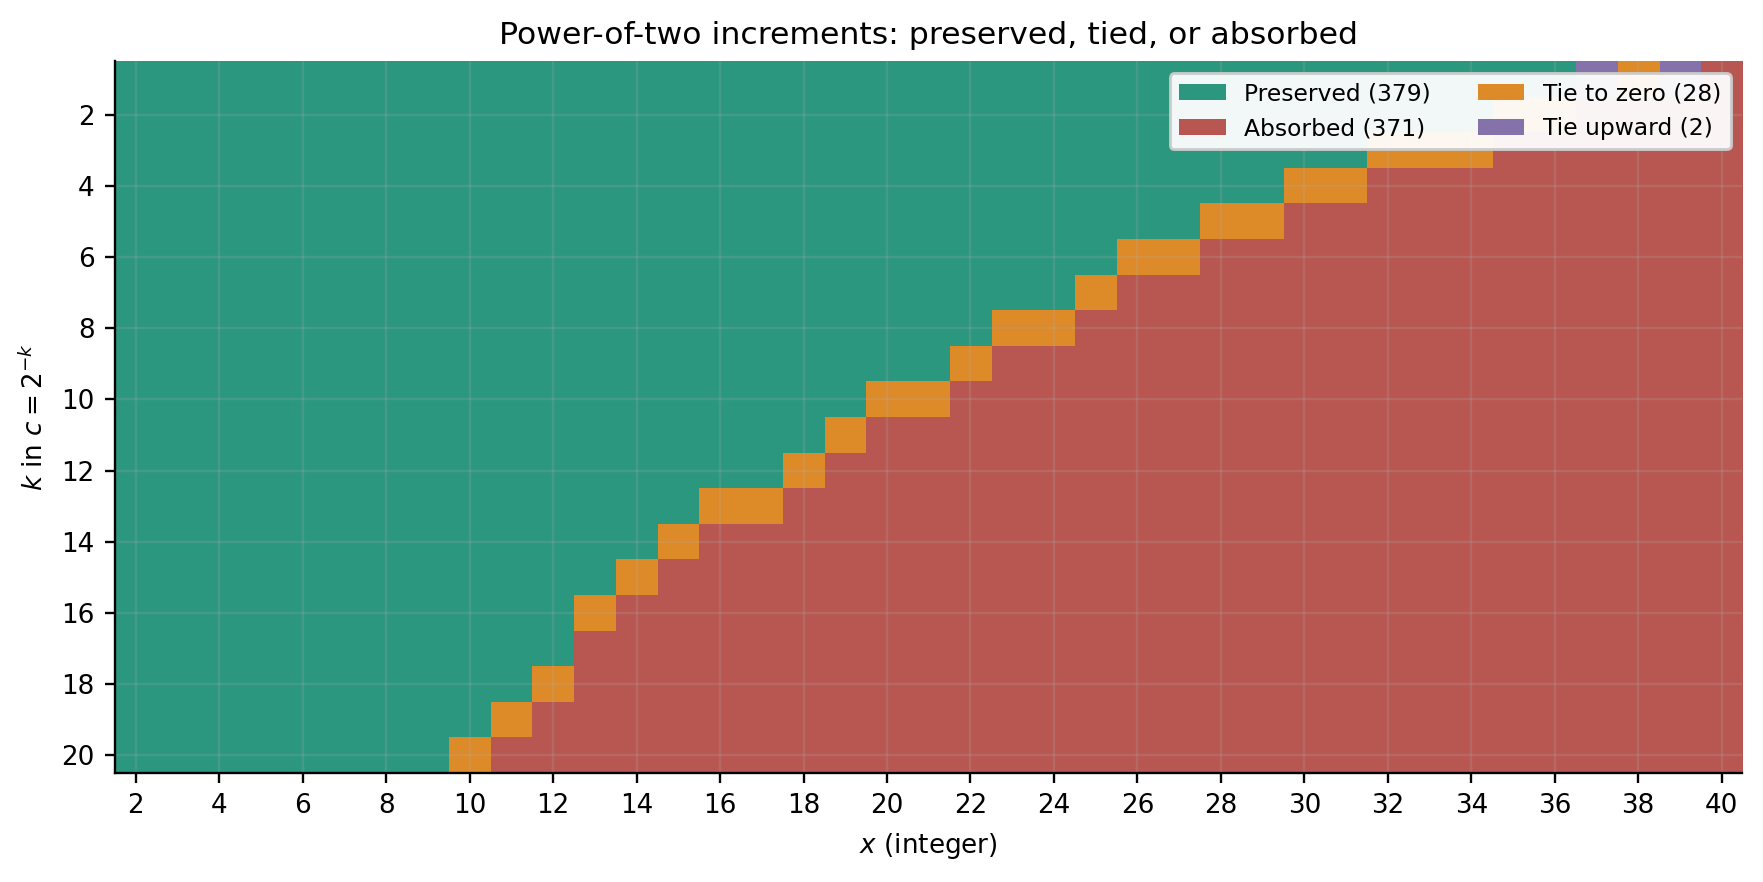
\includegraphics[width=.98\textwidth]{figs/02_power_two_map.png}
\caption{Power-of-two increment map on the 780-case integer grid. At a given $x$, smaller increments are absorbed; the narrow tie boundary separates preserved and absorbed results.}\label{fig:powmap}
\end{figure}

The 30 ties are not an implementation defect: both neighboring results are equally close to the exact sum, so ties-to-even selects according to the binary significand of $y$. Across a continuous $x$ grid, different sampled significands exhibit both possible tie outcomes. The observed transition zone for $c=2^{-1}$ is approximately $36.76\le x<39.40$; for $c=2^{-10}$ it is about $19.70\le x<21.11$, as described in the supplied preliminary report.

\begin{figure}[htbp]
\centering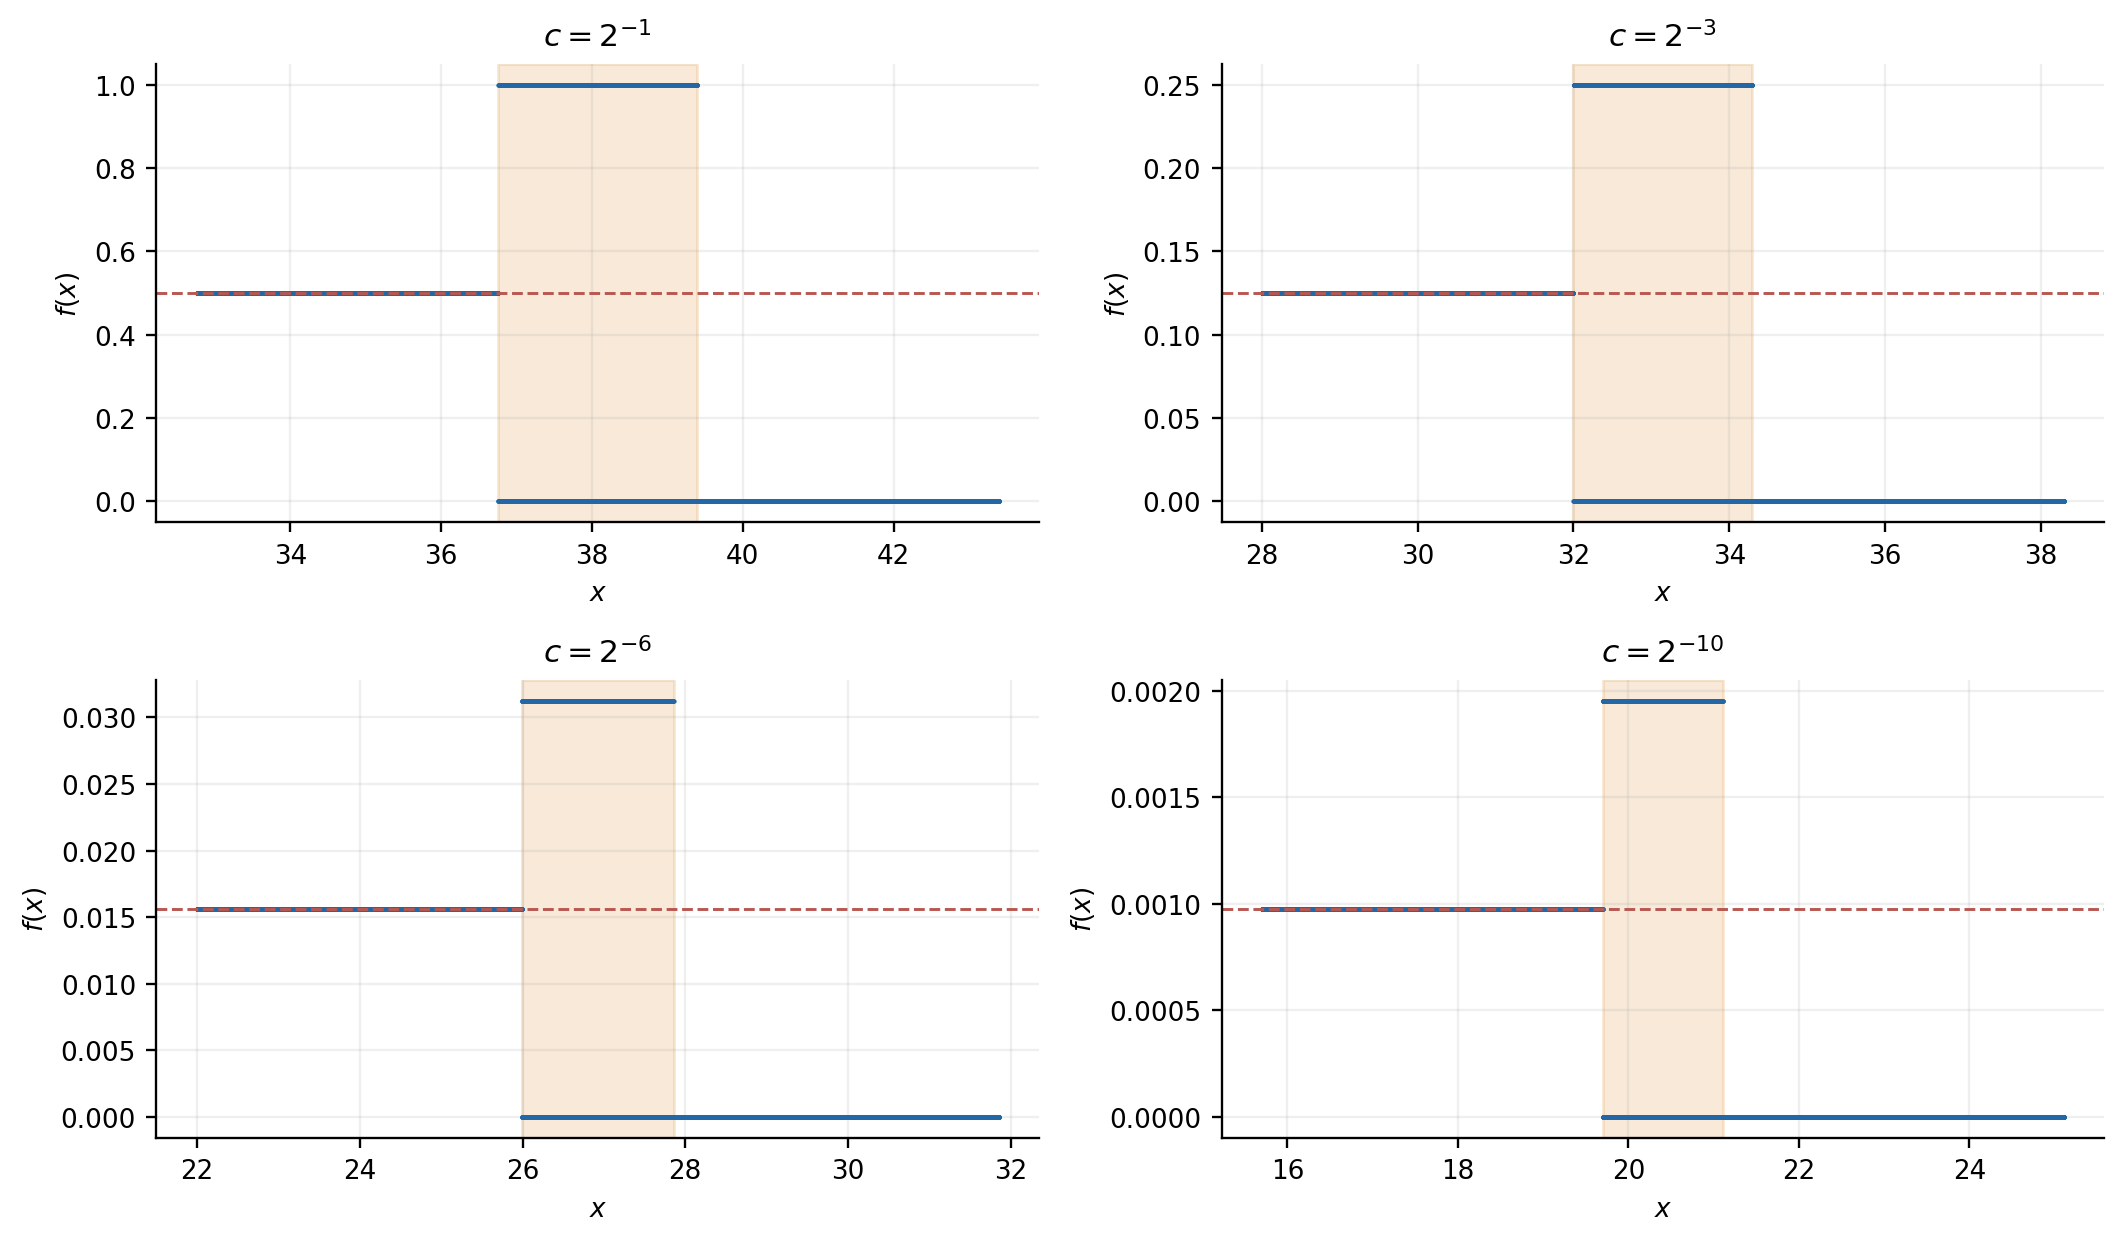
\includegraphics[width=.96\textwidth]{figs/03_power_two_curves.png}
\caption{Continuous numerical curves for $c=2^{-1},2^{-3},2^{-6},2^{-10}$ (binary64), corresponding to the supplied continuous Plotly experiments. The shaded strip identifies the parity-sensitive binade.}\label{fig:powcurves}
\end{figure}

\section{Odd integer increments}
For every positive odd integer $c$ representable in the chosen precision, $\nu(c)=0$. Therefore the onset of inexactness, when $y\ge c$ and binade crossing is excluded, does not depend on the \emph{value} of $c$: the first affected binade is $E=p$. For binary64 this begins near $x_1\approx39.40$, while for binary32 it begins near $x_1\approx5.28$. The end of the inexact zone does depend on the size of $c$ through $\lambda=\lfloor\log_2c\rfloor$.

\begin{table}[htbp]
\centering
\caption{Predicted first inexact and fully absorbed boundaries for selected positive odd integers, binary64. Values are rounded to two decimal places.}\label{tab:oddthreshold}
\begin{tabular}{rrrr}
\toprule
$c$ & $L$ (binades) & $x_1$ & $x_2$\\
\midrule
$1$ & 1 &39.40&42.22\\
$3$ & 2 &39.40&45.25\\
$5$ or $7$ &3&39.40&48.50\\
$21$&5&39.40&55.72\\
$101$&7&39.40&64.00\\
$1001$&10&39.40&78.79\\
$65537$&17&39.40&128.00\\
\bottomrule
\end{tabular}
\end{table}

At the first inexact binade, $u=2$ and every odd integer $c$ lies halfway between two multiples of two. The output is therefore $c-1$ or $c+1$. For all later interior binades, $u=4,8,16,\ldots$ and the computed increment changes by discrete jumps. In this regime $f$ is not necessarily monotonic in $x$; it can move above and below the exact value as different low-order bits of $c$ are discarded.

\begin{figure}[htbp]
\centering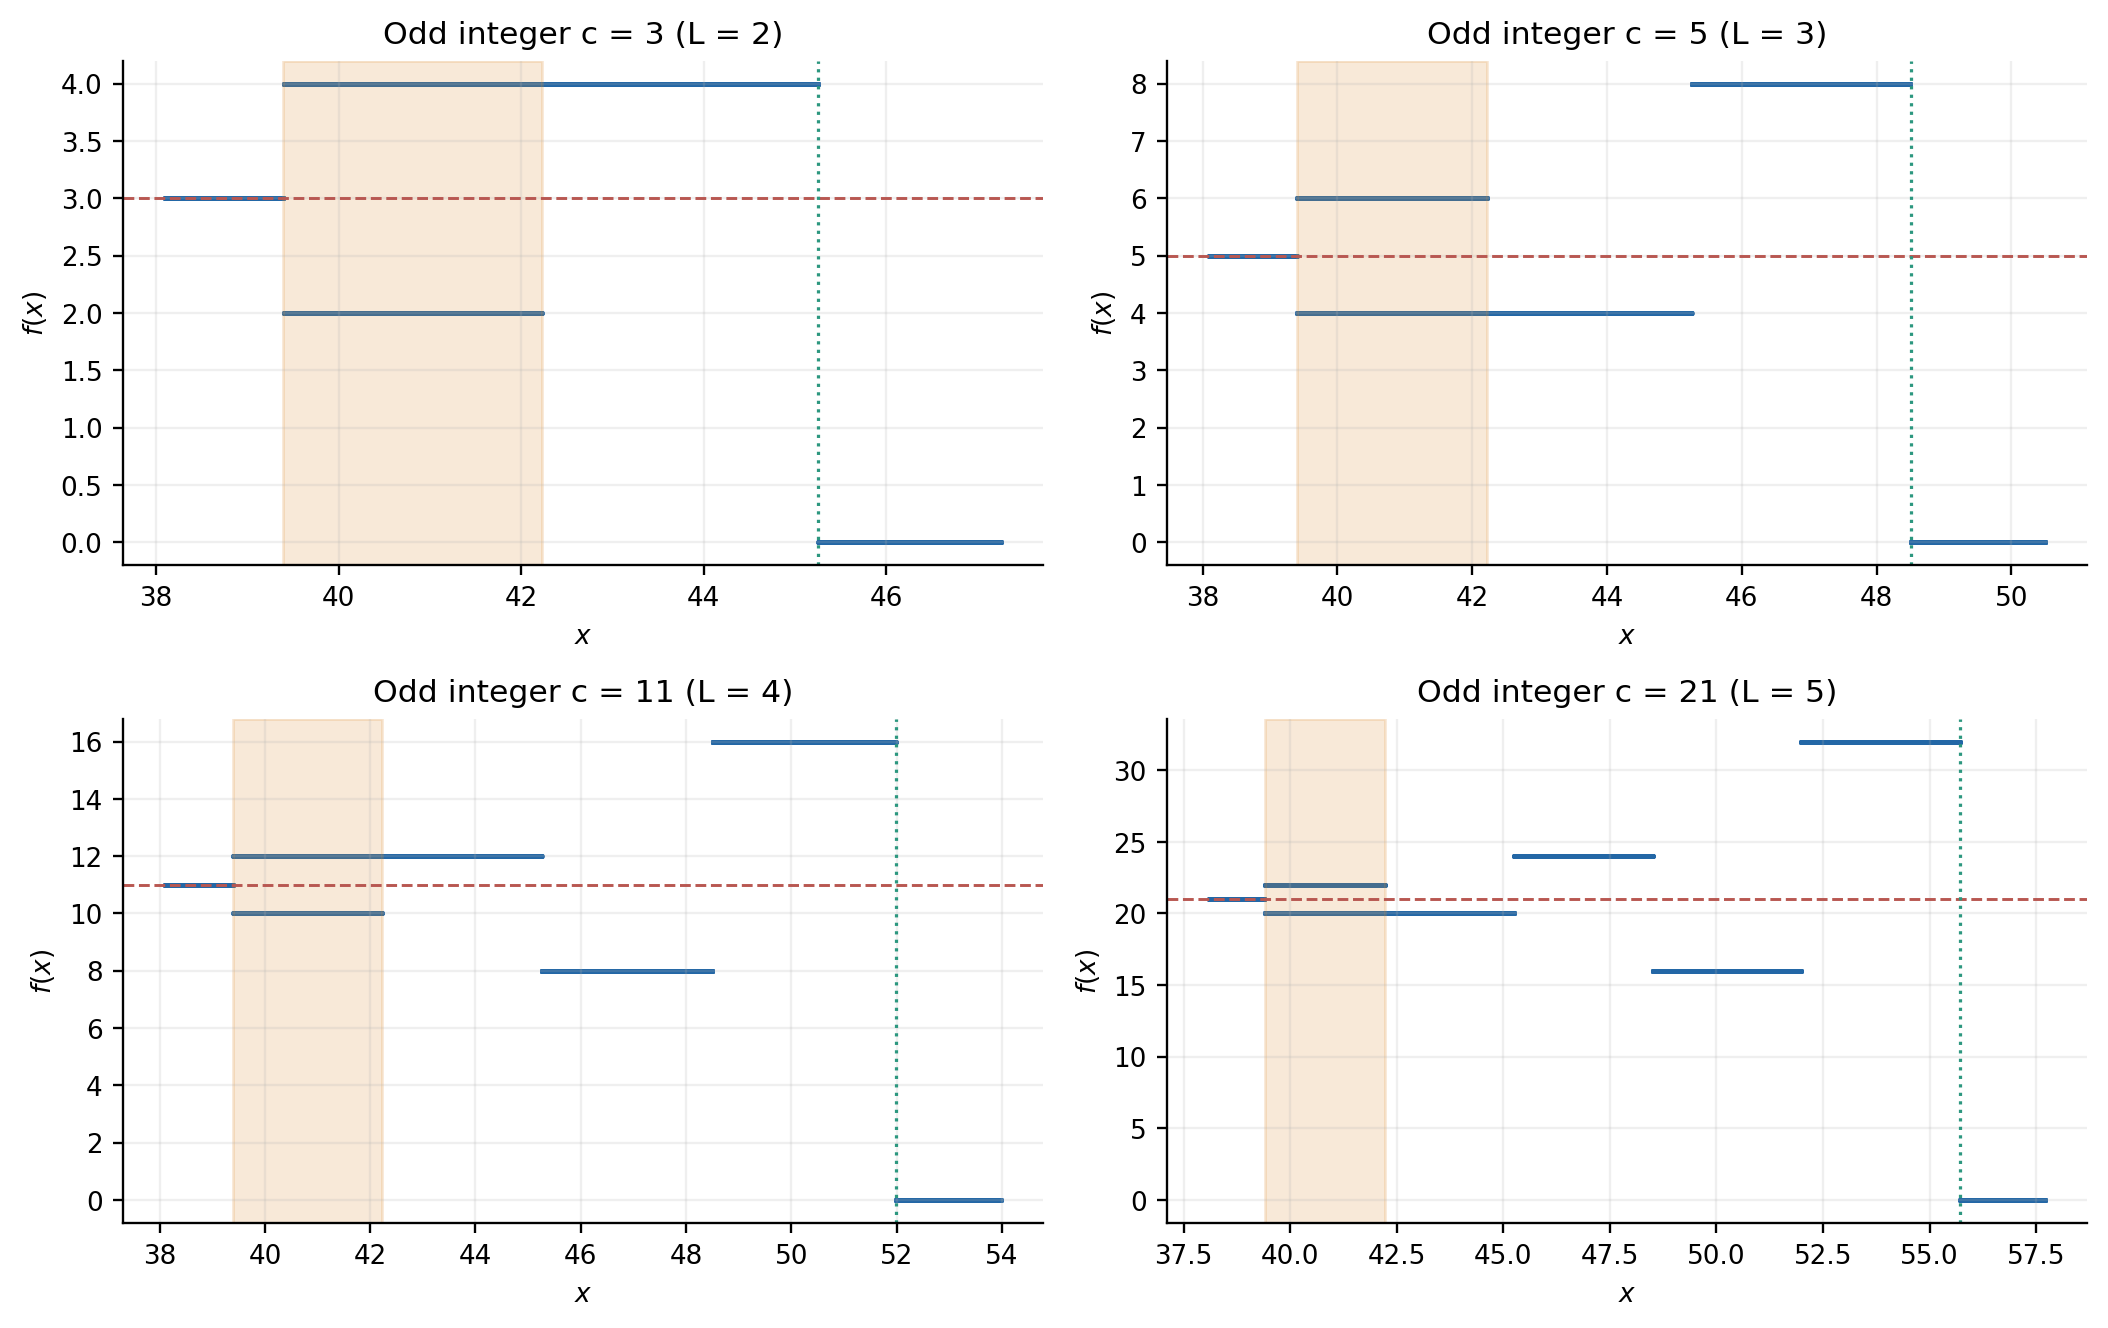
\includegraphics[width=.96\textwidth]{figs/04_odd_integer_curves.png}
\caption{Odd-integer experiments ($c=3,5,11,21$) reconstructed in English from the supplied family of Plotly curves. Dashed horizontal lines show the exact increment; dotted vertical lines mark the predicted complete-absorption boundaries.}\label{fig:oddcurves}
\end{figure}

For example, the manuscript presents $c=101$ as a particularly informative case. The output is $100$ or $102$ at $u=2$, then $100$ at $u=4$, $104$ at $u=8$, $96$ at $u=16$ and $u=32$, $128$ at $u=64$ and $u=128$, and $0$ from $u=256$ onward. The result $128$ represents a relative error $(128-101)/101\approx26.7\%$, despite being less than half of the ULP of $y$ in the relevant binade.

\begin{table}[htbp]
\centering\small
\caption{Model values for $c=101$ in binary64, taken from the supplied study. The tie binade has two possible values.}\label{tab:odd101}
\begin{tabular}{r r l r}
\toprule
Exponent $E$ & $u$ & Computed $f$ & Normalized error $\varepsilon$\\
\midrule
$E<53$ & $\le1$ & $101$ & $0$\\
$53$ & $2$ & $100$ or $102$ & $-0.5$ or $+0.5$\\
$54$ & $4$ & $100$ & $-0.25$\\
$55$ & $8$ & $104$ & $+0.375$\\
$56$ & $16$ & $96$ & $-0.3125$\\
$57$ & $32$ & $96$ & $-0.15625$\\
$58$ & $64$ & $128$ & $+0.421875$\\
$59$ & $128$ & $128$ & $+0.2109375$\\
$E\ge60$ & $\ge256$ & $0$ & $\le0$\\
\bottomrule
\end{tabular}
\end{table}

The heatmap in Figure~\ref{fig:oddheatmap} summarizes odd values from $1$ to $255$. Horizontal bands arise because $x_2(c)$ changes only when $c$ crosses a power of two, while the universal onset $x_1$ remains fixed. The drawn line gives the formula for the absorption threshold, not an independent fitted boundary.

\begin{figure}[htbp]
\centering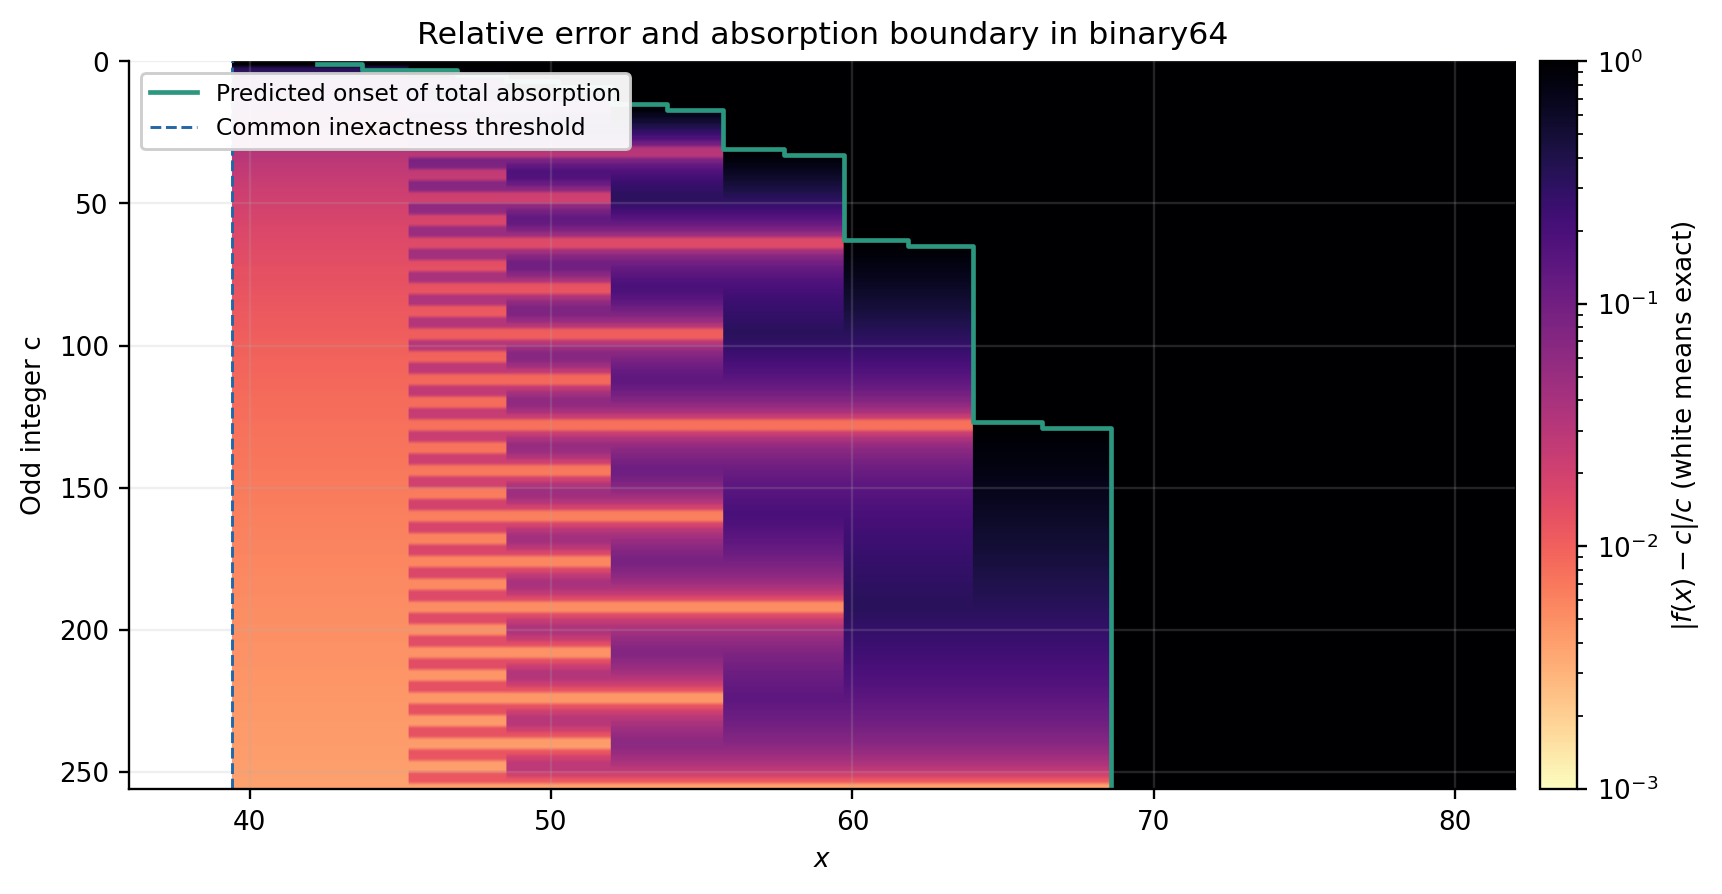
\includegraphics[width=.98\textwidth]{figs/05_odd_integer_heatmap.png}
\caption{Odd-integer relative error over a dense binary64 grid. The predicted complete-absorption boundary is superimposed on the numerical results.}\label{fig:oddheatmap}
\end{figure}

\section{Dyadic and non-dyadic fractional inputs}
Fractions of the form $m/2^j$ with odd $m$ are dyadic. Their first inexact binade is shifted by $j$ exponents compared with the same odd numerator: $\nu=-j$. Their width is still $L=\operatorname{bitlength}(m)$. For example, $c=3/4$ begins to round near $x_1\approx34.30$ and is fully absorbed from $x_2\approx39.40$; $c=5/16$ begins near $29.86$ and is fully absorbed from $36.76$.

An input such as decimal $0.1$ or mathematical $1/3$ is not dyadic. The value actually stored in a binary computer is a finite dyadic approximation and generally has many nonzero significand bits. For binary64, the stored value nearest decimal $0.1$ is $3602879701896397/2^{55}$, giving $\nu=-55$ and $L=52$. For the stored binary64 approximation to $1/3$, $L=53$. These large bit lengths imply a much longer region of affected binades than the power-of-two case.

\begin{table}[htbp]
\centering
\caption{Predicted inexact intervals for representative fractional increments. Inputs $0.1$ and $1/3$ denote their respective values after conversion to the indicated precision.}\label{tab:fractions}
\begin{tabular}{l rrr rrr}
\toprule
&\multicolumn{3}{c}{binary64}&\multicolumn{3}{c}{binary32}\\
\cmidrule(lr){2-4}\cmidrule(lr){5-7}
$c$ & $x_1$ &$x_2$ &$L$ & $x_1$ &$x_2$ &$L$\\
\midrule
$1/2$ &36.76&39.40&1&4.92&5.28&1\\
$3/4$ &34.30&39.40&2&4.59&5.28&2\\
$5/16$ &29.86&36.76&3&4.00&4.92&3\\
$0.1$ &0.87&32.00&52&0.81&4.29&24\\
$1/3$ &0.93&36.76&53&0.93&4.92&24\\
\bottomrule
\end{tabular}
\end{table}

\begin{figure}[htbp]
\centering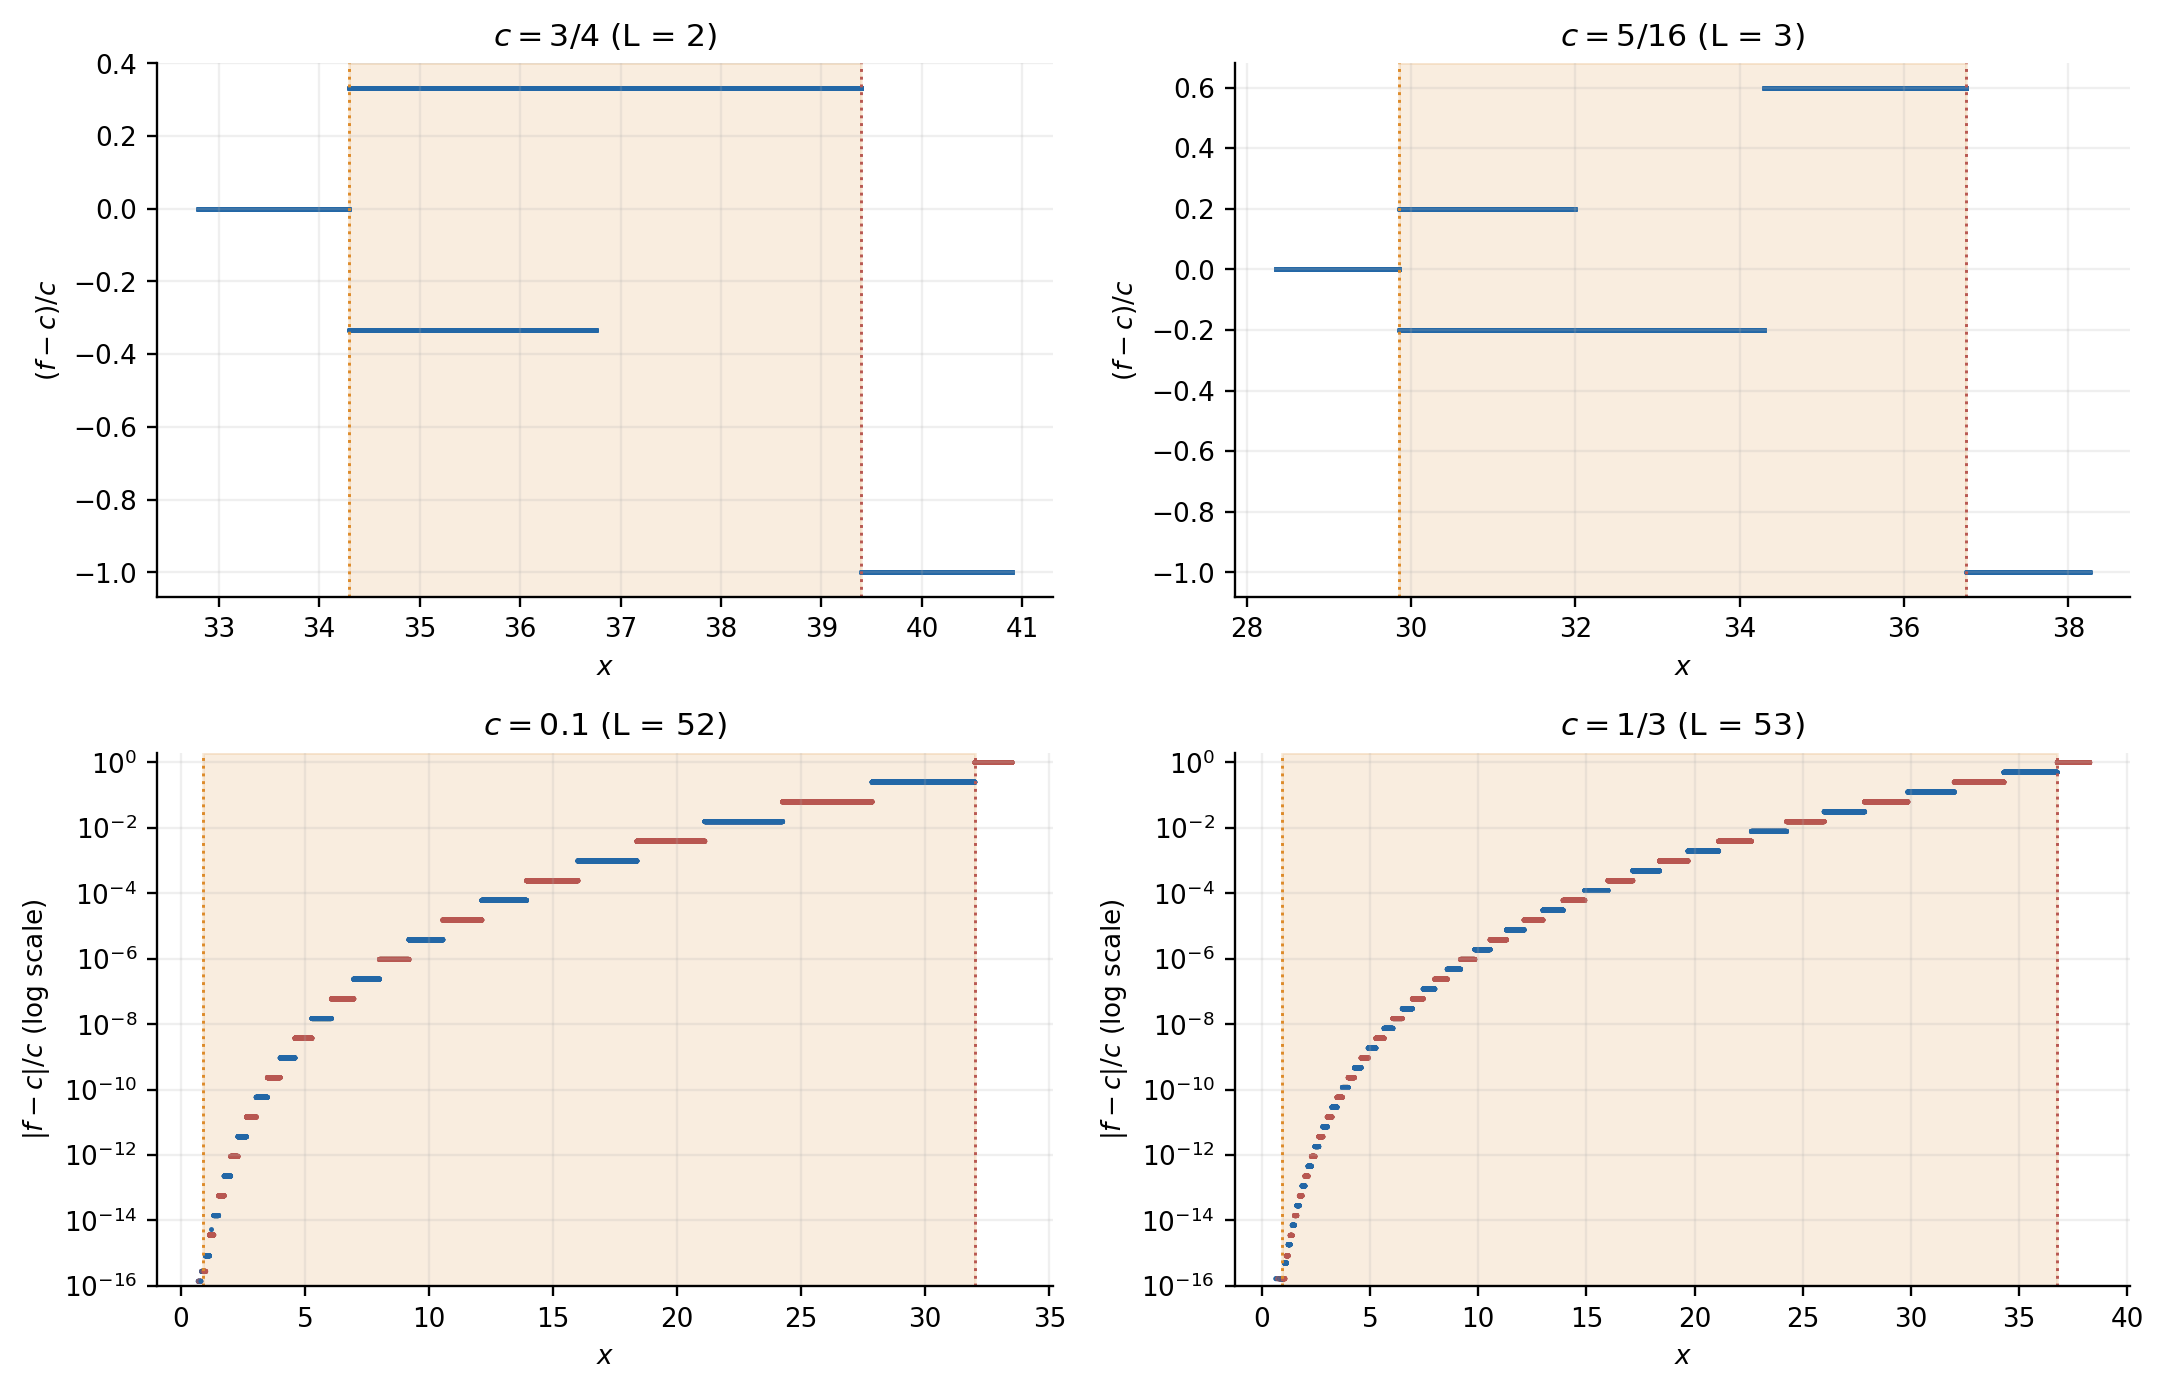
\includegraphics[width=.97\textwidth]{figs/06_fraction_behaviour.png}
\caption{Dyadic versus non-dyadic fractional increments in binary64. The lower panels show absolute relative error on a logarithmic vertical scale, exposing rounding long before absorption.}\label{fig:fractions}
\end{figure}

\begin{figure}[htbp]
\centering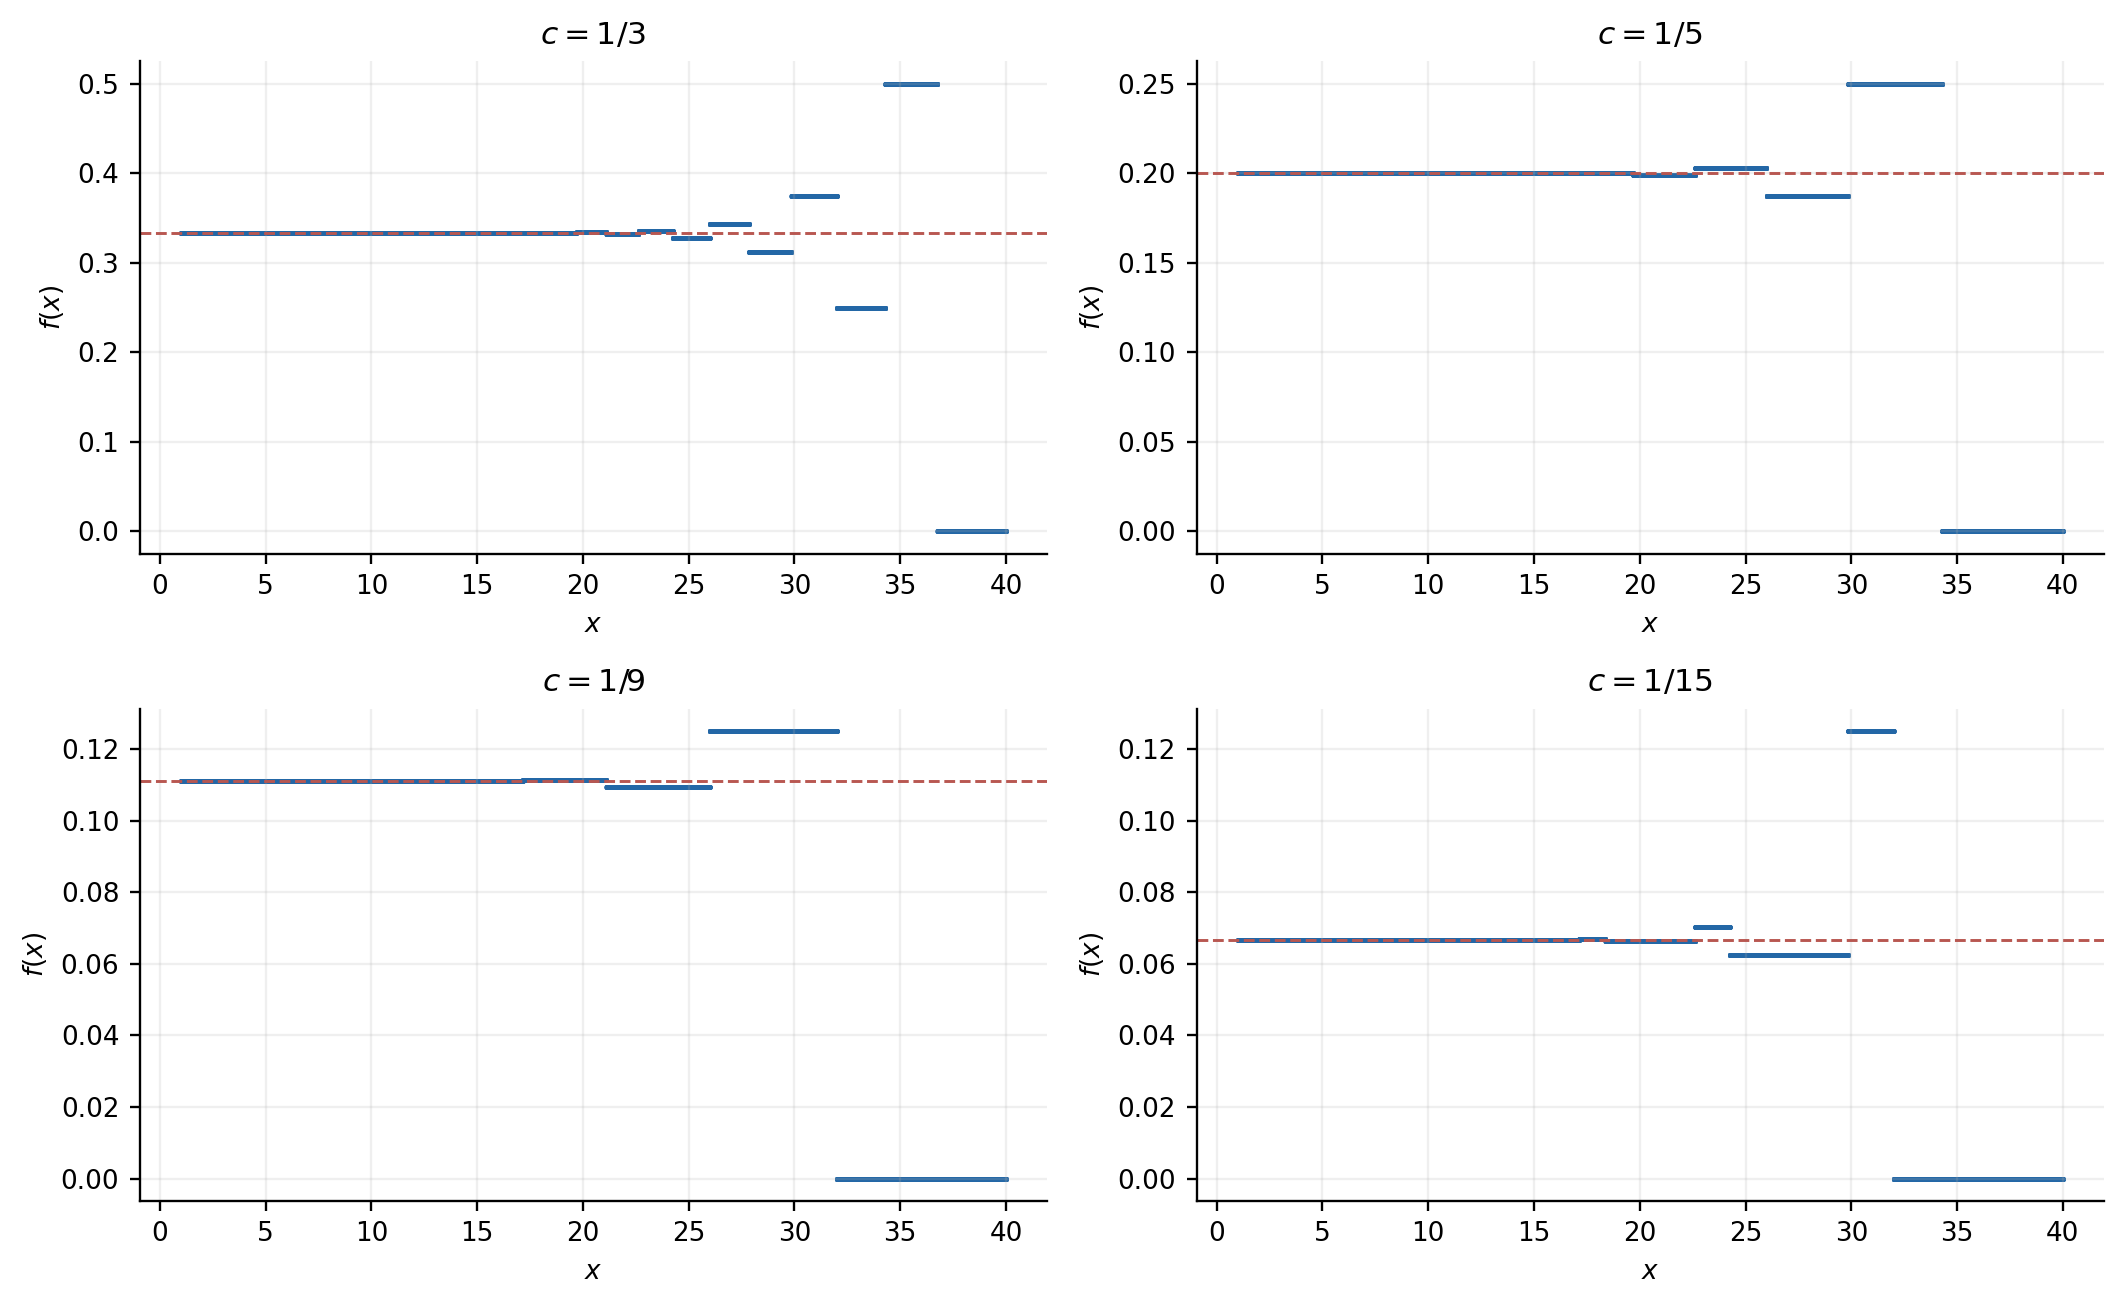
\includegraphics[width=.93\textwidth]{figs/09_reciprocal_odd_fractions.png}
\caption{Examples $c=1/d$ for selected odd denominators $d$ from the source's reciprocal-fraction Plotly experiment. The dashed line is the exact value $1/d$.}\label{fig:reciprocals}
\end{figure}

The supplied paper also reports relative errors for the stored approximations to $0.1$ and $1/3$ at selected binary64 inputs. Table~\ref{tab:relerr} reproduces these source measurements, with the convention that $(f-c)/c$ is measured relative to the \emph{stored} input $c$, not the ideal decimal constant. The relative error may be of order $10^{-9}$ at $x=5$, yet exceed $10^{-1}$ by $x=30$.

\begin{table}[htbp]
\centering
\caption{Relative errors $(f-c)/c$ reported in the source manuscript for binary64 fractions.}\label{tab:relerr}
\begin{tabular}{r rr}
\toprule
$x$ & $c=0.1$ &$c=1/3$\\
\midrule
$1$ & $+8.3\times10^{-16}$ &$-1.7\times10^{-16}$\\
$2$ & $-9.1\times10^{-13}$ &$-2.3\times10^{-13}$\\
$5$ & $-3.7\times10^{-9}$ &$+1.9\times10^{-9}$\\
$10$ & $+3.8\times10^{-6}$ &$+1.9\times10^{-6}$\\
$20$ & $-3.9\times10^{-3}$ &$+2.0\times10^{-3}$\\
$30$ & $+0.25$ &$+0.125$\\
$32.5$ & $-1$ &$-0.25$\\
\bottomrule
\end{tabular}
\end{table}

\section{Comparison between binary32 and binary64}
The same model applies to both IEEE 754 formats after replacing the precision $p$. For odd integers, the first affected $x$ decreases from approximately $39.40$ in binary64 to $5.28$ in binary32. The number $L$ of affected binades is unchanged for an exactly representable $c$ shared by both formats. For common non-dyadic literals, on the other hand, the binary32 approximation typically carries only about 24 relevant bits rather than about 53, and its predicted inexact interval is correspondingly narrower in log-space.

\begin{figure}[htbp]
\centering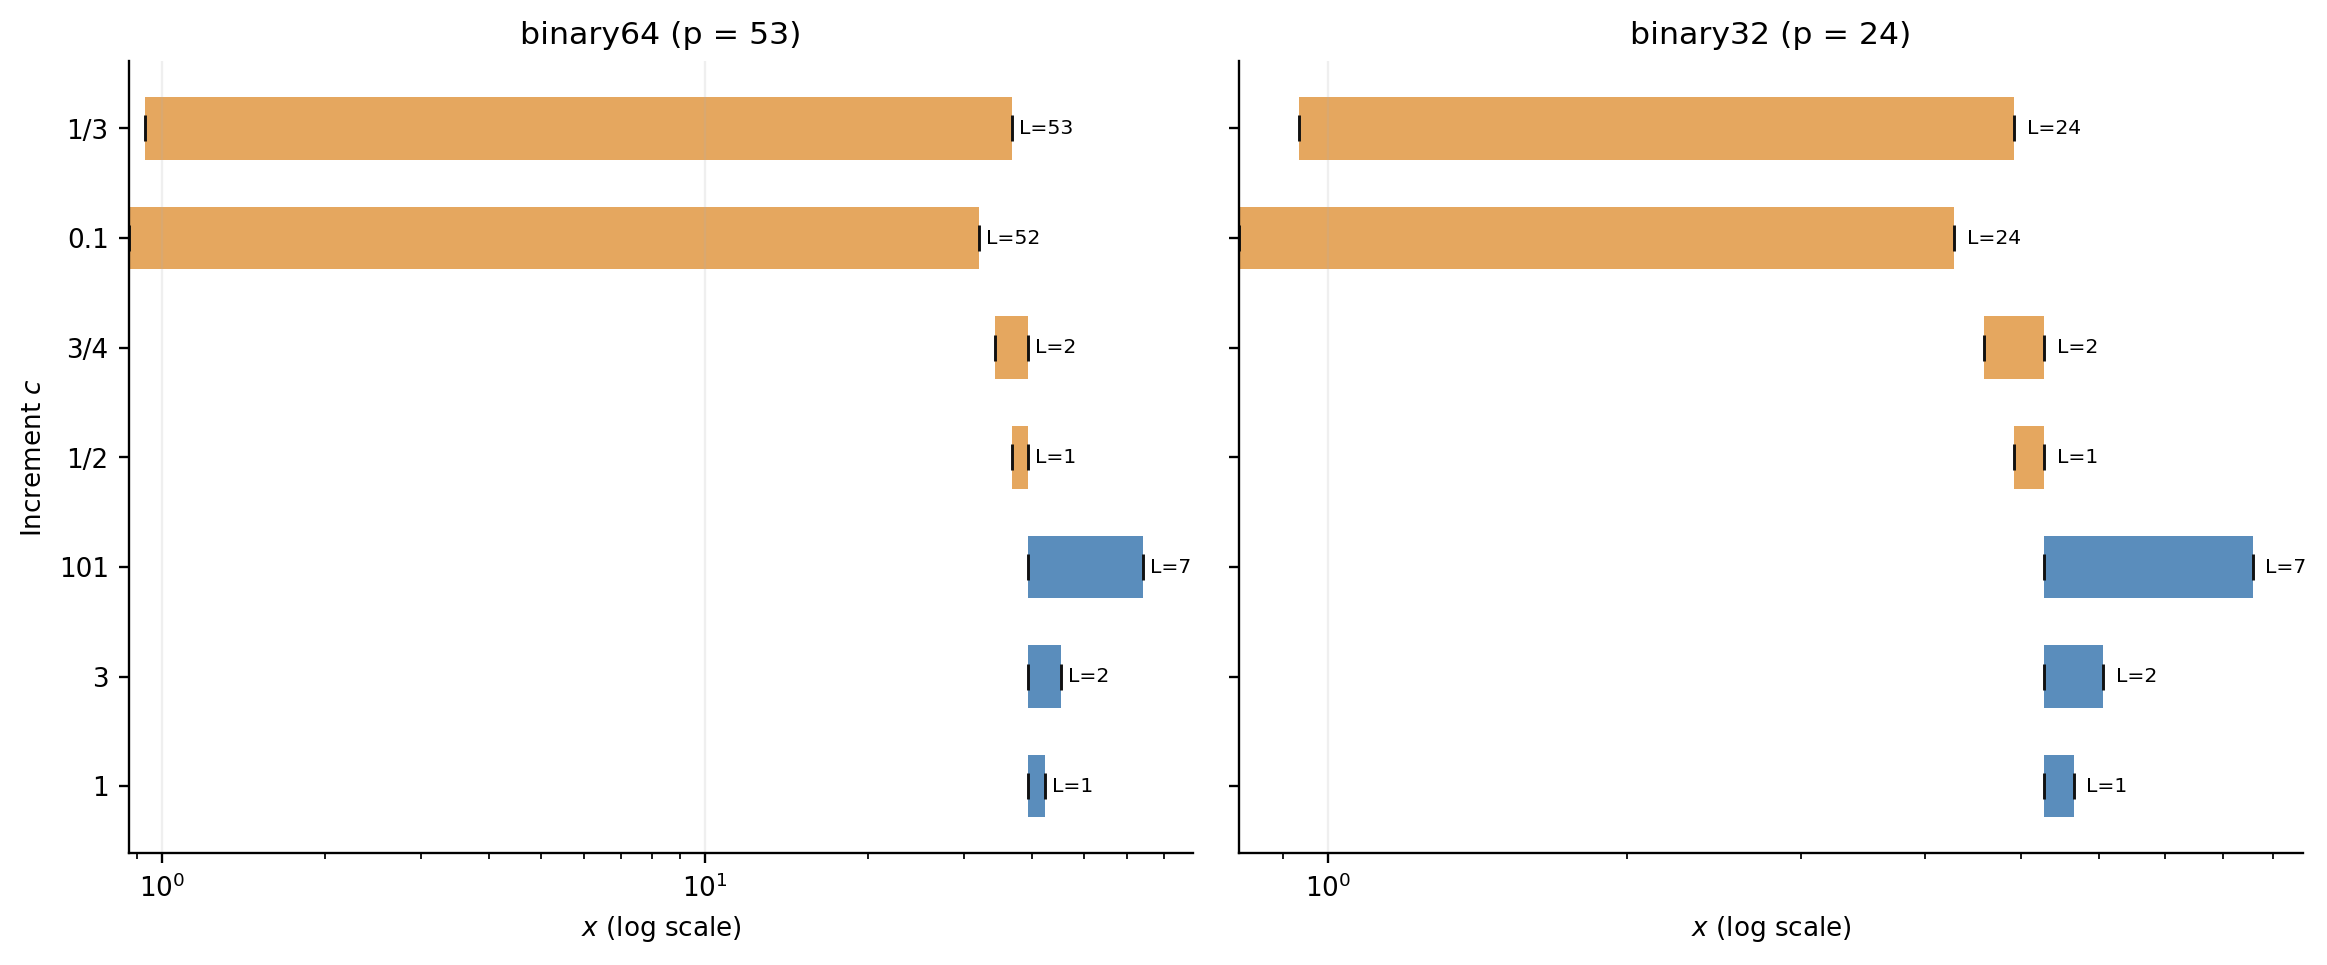
\includegraphics[width=.98\textwidth]{figs/07_precision_comparison.png}
\caption{Predicted inexact ranges in the two precisions for representative increments. The bars visualize the formulas for $x_1$ and $x_2$; they are not uncertainty intervals.}\label{fig:precision}
\end{figure}

The source study reports that the nearest-grid model matched its 1,611 tested increments in each precision after accounting for samples outside the model's domain (including binade crossings). These are reported outcomes from the original validation scripts. A particularly useful practical warning is that an input $c$ may itself change when converted to binary32; comparisons must therefore use the \emph{represented} $c$ in each format rather than assume that the same exact real increment is available to both.

\chapter{Discussion and Limitations}\label{ch:discussion}

\section{Why a small ULP error can be a large relative error}
The nearest-grid result contains an important numerical distinction. Equation~\eqref{eq:eps} limits the addition's rounding error to $u/2$ in the interior of a binade, but the ULP $u$ belongs to the large quantity $y\approx x^{10}$, not to the small increment $c$. As $x$ increases, $u$ doubles every time $x$ grows by a factor $2^{1/10}\approx1.072$. With $c$ fixed, an error small on the scale of $y$ may be larger than the quantity one is trying to recover. Complete absorption occurs when the stored sum is identical to $y$, so the final subtraction gives exactly zero.

A subtle issue of terminology is that this expression involves both \emph{absorption during addition} and \emph{subtraction of nearby values}. The observed loss can occur even though the subtraction itself is exact. It is therefore more precise to attribute the loss in the model regime to rounding the addition, not to claim that Sterbenz's exact subtraction creates the error. This follows the error-analysis perspective of standard floating-point treatments \cite{goldberg1991floating,higham2002accuracy}.

\section{Binade crossings and the region below \texorpdfstring{$c$}{c}}
The main proposition assumes $y+c$ is smaller than the next power of two. For the small fraction of inputs very close to that boundary, the sum lands in a binade with twice the spacing; a one-ULP-of-$y$ error bound replaces the interior half-ULP bound. The extended source draft explicitly distinguishes a proved bound from a heuristic for the frequency of this effect. It reports no such crossings among $4\times10^7$ sampled binary64 cases for odd or dyadic increments in the noisy region, 82 occurrences among the corresponding $4\times10^7$ binary32 cases, and approximately $0.3\%$ and $1\%$ for non-dyadic increments in binary64 and binary32, respectively. These reported frequencies are sampling results, not probabilities deduced exactly from the model.

At small $x$ when $y<c$, Sterbenz's criterion may fail. The draft bounds the deviation by $2\ulp(c)$ and reports smaller deviations (at most one ULP of $c$) in the observed samples. Consequently, the familiar summary ``exact, then noisy, then zero'' should be read as a statement about the regular regime $y\ge c$ away from binade crossings; it is not an unconditional theorem for the entire positive real line.

\section{Input conversion and computation order}
Decimal literals such as \code{0.1} introduce a separate representation error before the experiment starts. In this report, $f-c$ means an error relative to the stored, exactly specified binary value of $c$. The error relative to the ideal real input is the sum of this conversion effect and the subsequent arithmetic effect. Likewise, evaluating $y=x^{10}$ with \code{pow}, repeated multiplication, or exponentiation by squaring can produce slightly different stored values. The nearest-grid reasoning applies to each resulting $y$, but the $x$ positions of transitions may move. The submitted sources do not provide a controlled comparative benchmark of all these evaluation paths; none is invented here.

\section{Connection with Fast2Sum and possible remedies}
The intermediate result in Fast2Sum has the form
\begin{equation}
 s=\fl(y+c),\qquad z=\fl(s-y),\qquad t=\fl(c-z).
\end{equation}
Our computed function is exactly $z$ under the same operation order. Error-free transformations such as Fast2Sum and TwoSum use additional operations to represent the residual of a floating-point addition, rather than discard it \cite{dekker1971technique,knuth1997seminumerical}. When the algorithm's hypotheses hold, the pair $(s,t)$ represents the exact sum $y+c$. This connection is already present in classical numerical-arithmetic literature; the supplied study's contribution is to express the intermediate $z$ through $\nu(c)$, $\lambda$, and the $x$-thresholds.

For this \emph{specific} mathematical identity, the best remedy is algebraic: compute $c$ directly, without forming a large intermediate sum and subtracting it back. In less trivial computations, avoiding unnecessary cancellation, retaining a rounding residual when appropriate, and understanding compiler evaluation order are the more general lessons. A comparison of compensated summation methods is suggested by the source draft, but no new experimental claims about those methods are made here.

\section{What is proved, observed, and open}
The underlying proof rests on representable-grid rounding and the exactness of sufficiently close subtraction. Within the explicitly stated domain, Equations~\eqref{eq:grid}--\eqref{eq:xthreshold} are theoretical consequences; the half-ULP normalized error bound is also proved. The 780-case heatmap and plotted curves are local replications. The broader 1,611-input validation and the rare-crossing frequencies were reported by the supplied research sources.

Further work identified by the source authors includes the behavior for negative $c$, the exact distribution of binade-crossing events, precise bounds in the $y<c$ region, alternative ways of evaluating the power, fused or extended intermediate arithmetic, and extension to other precisions. The research draft also cautions against presenting the threshold notation as a demonstrated novelty without a more complete literature review, since the relevant exact-subtraction and error-free-transformation mechanisms are already established \cite{rocha2026bookdraft}.

\chapter{Conclusions}\label{ch:conclusion}
The numerical behavior of $(x^{10}+c)-x^{10}$ can be understood through the ULP of the reused stored power $y$ and the low-order binary structure of the stored increment $c$. Away from binade crossings and with $y\ge c$, the output equals the increment rounded to the nearest multiple of $\ulp(y)$, with ties determined by the parity of the significand of $y$. This produces an initial exact regime, a parity-sensitive first inexact binade, discrete rounded plateaus, and complete absorption.

Writing $c=m2^{\nu}$ with odd $m$ and $\lambda=\lfloor\log_2c\rfloor$, the model predicts $x_1\approx2^{(p+\nu)/10}$ and $x_2\approx2^{(p+1+\lambda)/10}$, with $L=\lambda-\nu+1$ potentially inexact binades. The distinction between one-bit increments and long-significand fractions explains why powers of two produce narrow transition bands whereas stored approximations to values such as $0.1$ or $1/3$ show error over a much broader range. In binary64, odd integers first become inexact near $x=39.40$; in binary32 the corresponding point is near $x=5.28$.

The supplied study reports a 1,611-increment validation in each precision, while the independently repeated 780-case power-of-two classification agrees with the preliminary report. Explicit assumptions and the exceptions at binade boundaries remain necessary. The example is pedagogically valuable because it exposes a key floating-point principle: an operation can be perfectly well rounded relative to its \emph{large} operand and still completely destroy the information in its \emph{small} operand.

\printbibliography
\appendix
\chapter{Reproducibility and Source Notes}\label{app:rep}

\section{Generating the figures}
From the directory containing \code{func\_nummet\_report.tex}, run:
\begin{verbatim}
python -m pip install numpy matplotlib
python scripts/generate_figures.py
latexmk -pdf -interaction=nonstopmode func_nummet_report.tex
\end{verbatim}
The plotting script regenerates all nine English-language PNG files in \code{figs/}. The original experiments represented in the supplied source documents used NumPy and, for the interactive charts, Plotly. An English-commented adaptation of the source validation code is available at \code{scripts/source_validation/validate.py}; its full run is considerably more demanding than figure generation.

\section{Source-material inventory}
The supplied inputs comprised one LaTeX template archive; an extended Portuguese-language manuscript and corresponding source archive; an eight-page research article; a seven-page preliminary experimental report; a Jupyter notebook; and four interactive Plotly HTML visualizations (power-of-two grid, continuous power-of-two curves, odd integers, and odd reciprocals). The current document is an English synthesis of those supplied materials; it is not a verified independent replication of every experiment in the manuscript.

\section{Source attribution and publication status}
The supplied main article and book draft identify Lucas Martins Rocha as their author, and this report retains that attribution. The notebook originally extends material attributed in the supplied research manuscript to E.~R.~L.~D.~Ribas, \code{numError01}, under an MIT license. The template did not provide a verified supervisor or institutional affiliation for the author of the new report. Accordingly, no supervisor was inferred. The provided class and cover design are retained as a layout template; any institution-specific branding should be confirmed before external publication.

\section{Assumptions checklist}
The theoretical results should be applied only after checking: (i) finite positive stored $c$; (ii) normal finite values and no exception-producing overflow/underflow; (iii) round-to-nearest, ties-to-even; (iv) a single stored value of $y$ reused; (v) no fused or extended-precision rearrangement; and, for the nearest-grid formula as stated, (vi) $y\ge c$ and $y+c<2^{E+1}$. If these conditions are not met, the source manuscript analyzes some cases separately and identifies others as open.

\end{document}
